\documentclass[12pt, letterpaper]{article} % Defines document type, font size, and paper
\usepackage[utf8]{inputenc}                % Sets input encoding (standard)
\usepackage[T1]{fontenc}                   % Sets font encoding for better output
\usepackage[english]{babel}                % Sets language
\usepackage{geometry}                      % For adjusting page margins
\usepackage{graphicx}                      % For including graphics and images
\geometry{margin=1in}                      % Sets all margins to 1 inch
\usepackage[
backend=biber,
style=numeric,
]{biblatex}
\addbibresource{references.bib}

\title{Non-Parametric Statistics, the Mann-Whitney U-Test and the Kruskal-Wallis Test}

\begin{document}
\maketitle % Generates title, author, and date

The statistical paradigms learned when beginning statistics are typically parametric. T-tests, any kind of regression, most of what we call ``machine learning'' --- all of this is parametric. Both classical statistical paradigms, Bayesian and Frequentist find themselves embroiled in parametric statistics. In contrast we have nonparametric statistics. While the definition of non-parametric is up for debate, here we use the definition given by Siegel\cite{siegel1957nonparametric}, which is simply that these methods don't assume a distribution in their calculation. This is all important in the context of hypothesis testing, where we have experimental data and want to report a statistical outcome. In a field like neuroscience, where we might not really know how something like time spent grooming is distributed, this is very powerful. The below figure shows hypothesis testing under the assumption of the normal distribution, which is an example of parametric statistics. The normal has two parameters, $\sigma$ and $\mu$, which control the variance and mean respectively.

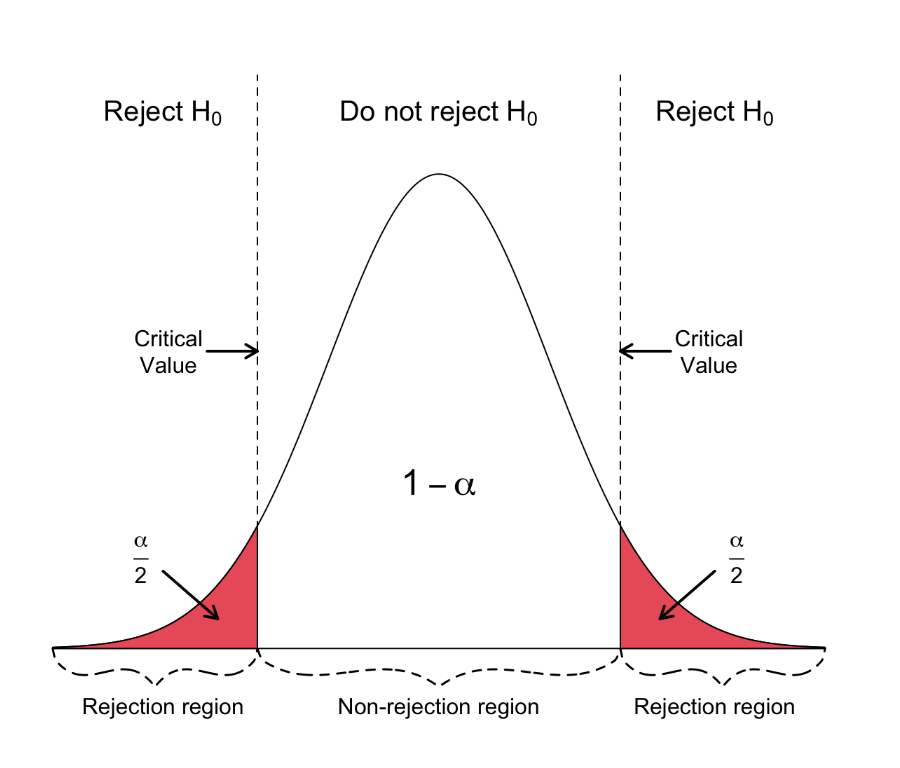
\includegraphics[width=0.5\textwidth]{images/normal.png} 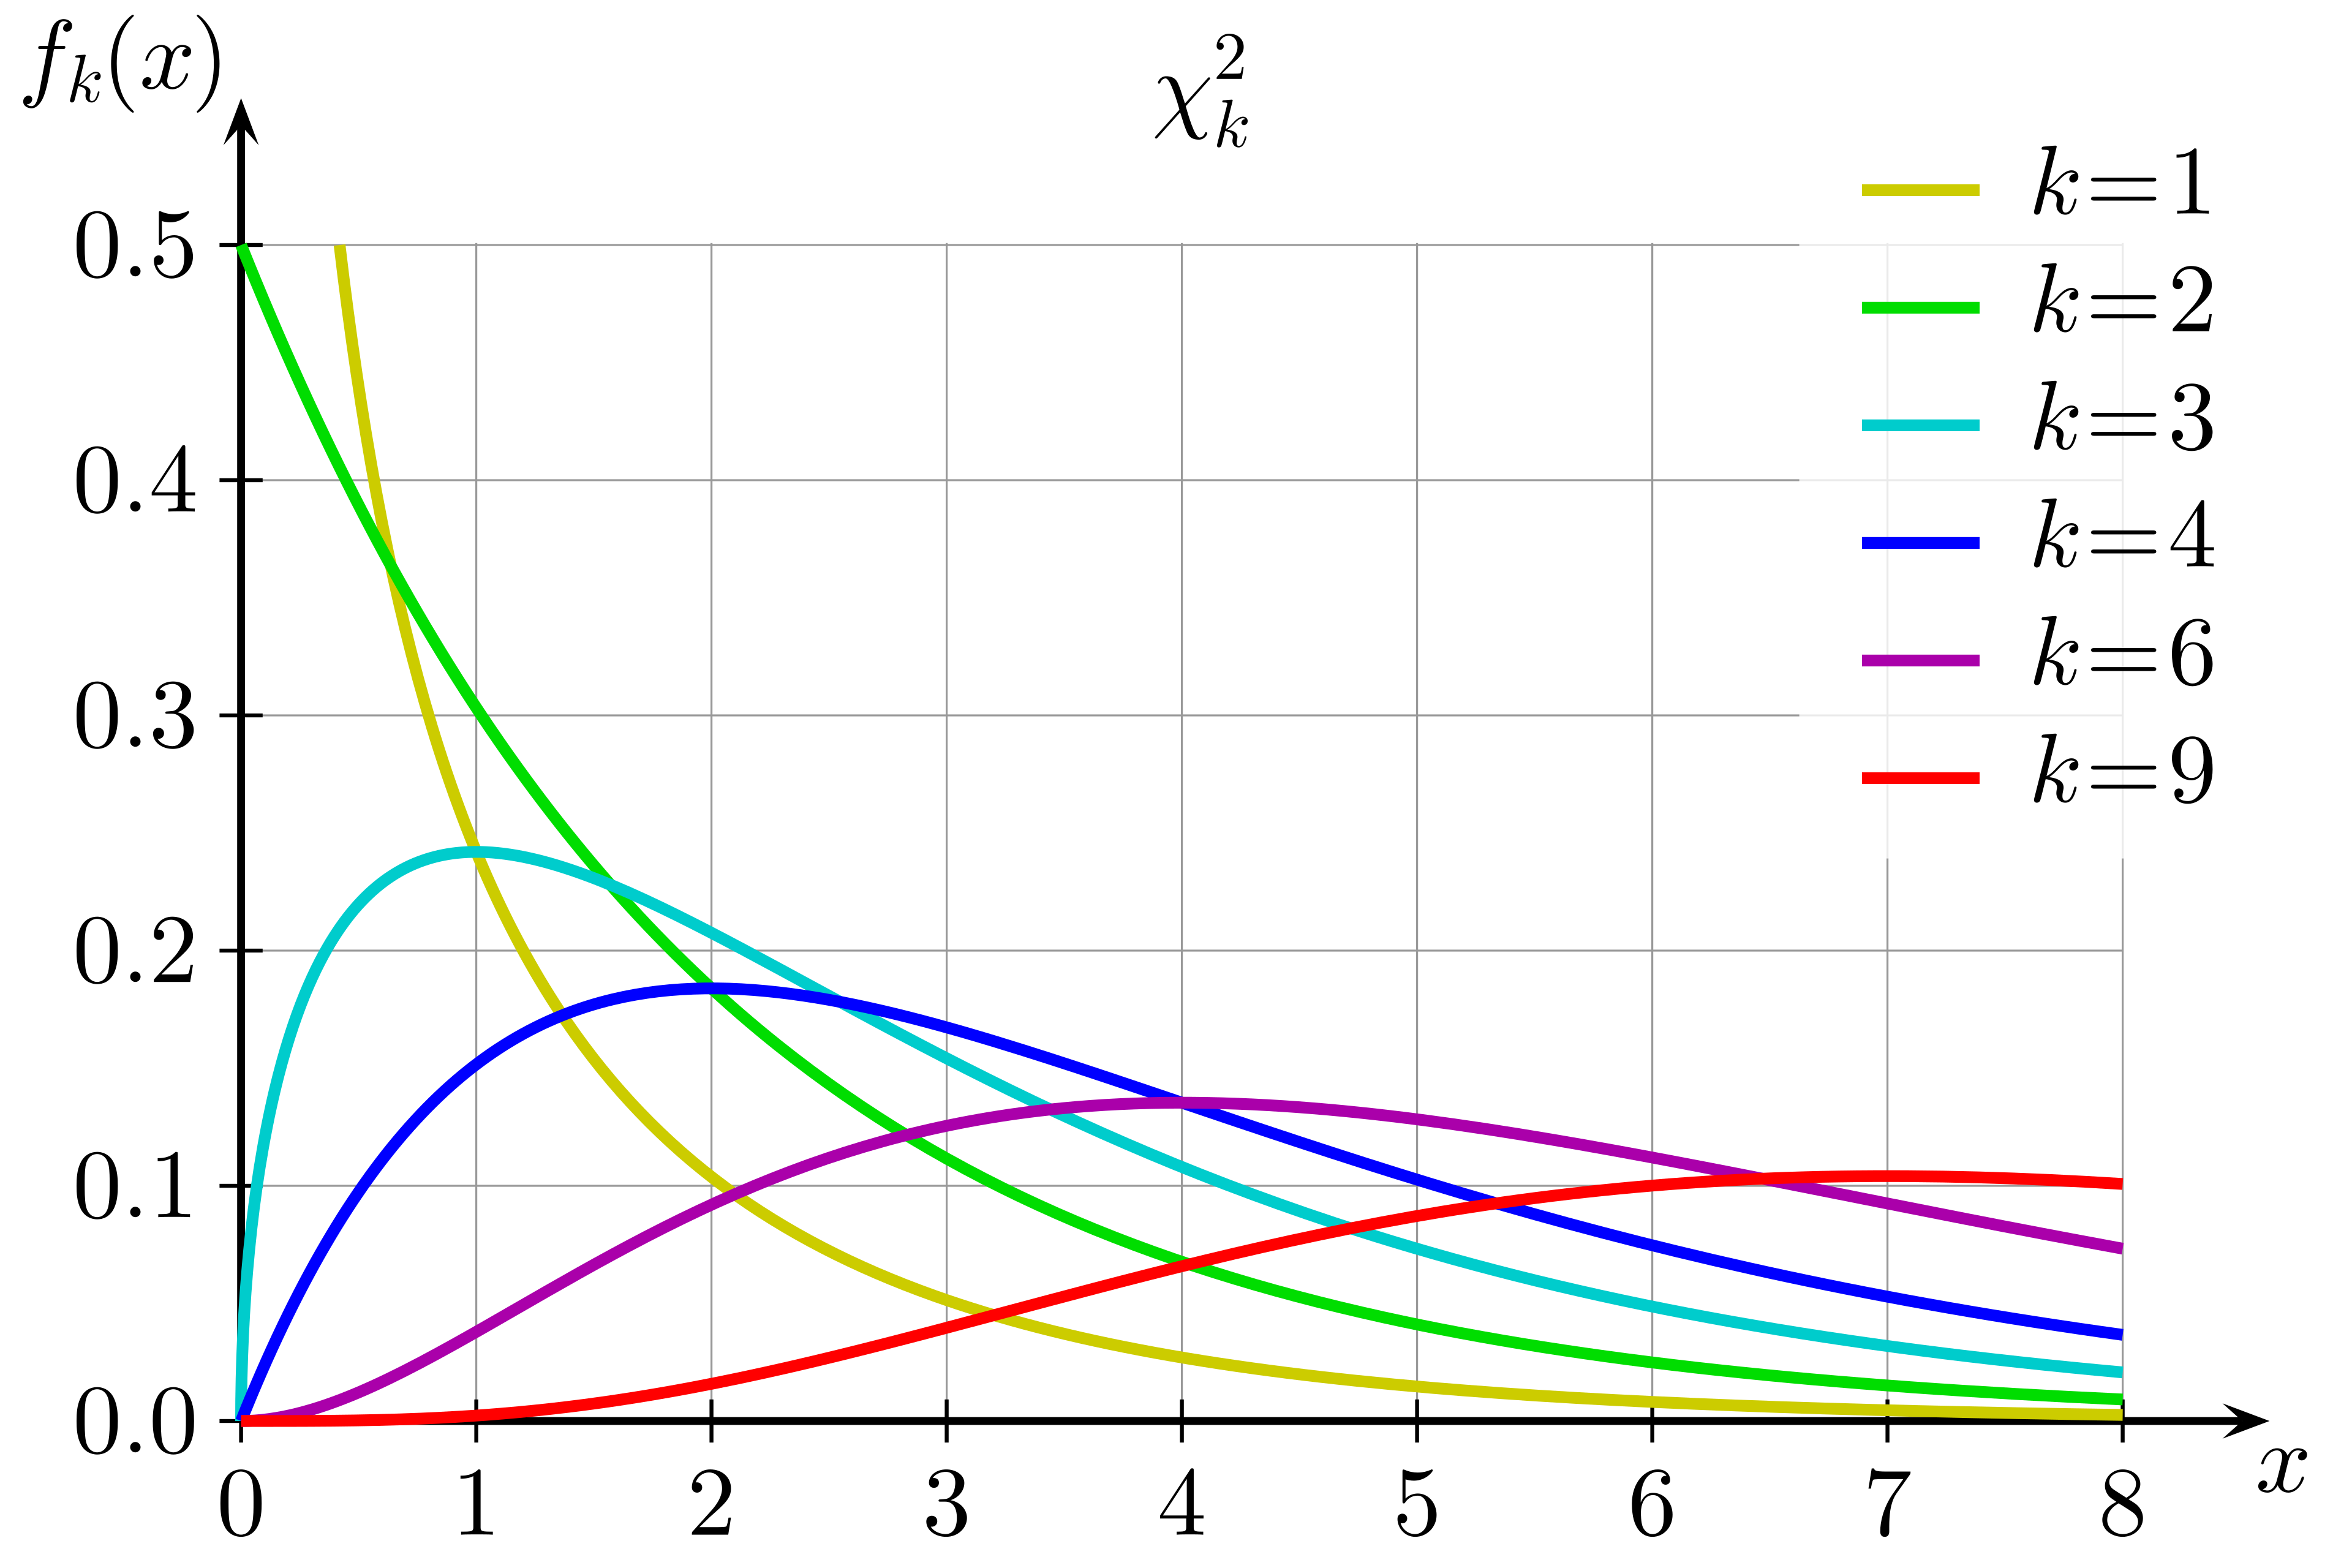
\includegraphics[width=0.5\textwidth]{images/chisquare.png}

How does this work? In practice its actually a little more complicated than parametric statistics, where we get to use concepts like maximum likelihood estimation to make claims about our data. In nonparametric statistics, we use an algorithm to calculate what is ultimately an abstract metric. The distribution of this metric may be known, but it has no correspondence to the distribution of the data. The Kruskal-Wallis test statistic is ususally treated as chi-square distributed, as above. In neuroscience, we see the Mann-Whitney U-Test (Wilcoxon Rank Sum Test) and Kruskal-Wallis test used in conjunction for hypothesis testing. Both tests are built up from the idea of ranking in distributions and carry similar assumptions. The tests assume the data is ordinal and independently distributed. Ideally for both tests, we have identically distributed and scaled populations, as the test is more powerful in this case.

In the Mann-Whitney U-Test, the null hypothesis is that the two distributions are identical. If they are scaled and dispersed the same with only a shift in location, then significance in the test makes a claim about the medians as well. We calculate the U statistic as follows:

\begin{equation}
    U_1 = n_1n_2 - \frac{n_1(n_1+1)}{2} - R_1, \quad U_2 = n_1n_2 - \frac{n_2(n_2+1)}{2} - R_2
\end{equation}

The lesser of these two is the U statistic, the likelihood of which is given by either a normal approximation or exact calculation based on combinatorics. This is best thought of as one distribution stochastically dominating the other. If the test is significant, it is more likely than not that if a value is chosen at random from the upper distribution it is higher than a value chosen at random from the lower. Importantly, the U statistic is based on ranks, not the true values, which means we lose some specificity in its calculation.

The Kruskal-Wallis Test extends the Mann-Whitney U Test for cases where we want to make a statement about more than two populations. The assumptions are the same but we now increase the chance of making a Type I error due to differences in scale and dispersion. We calculate the H statistic as follows:

\begin{equation}
    H = (N-1)\frac{\sum^g_{i = 1}n_i (\bar r_i - \bar r)^2}{\sum_{i=1}^g\sum_{j=1}^{n_i}(r_{ij}\bar r)^2}
\end{equation}

Conveniently, it's chi-squared distributed with $g-1$ degrees of freedom so we can easily calculate a p-value. It doesn't tell us about pairwise comparisons, so frequently researchers apply the post-hoc Mann-Whitney U Test. In this case, we're making so many comparisons that it's a good idea to apply the Bonferroni correction to our $\alpha$ as follows:

\begin{equation}
    \bar \alpha = \frac{2\alpha}{g(g-1)}
\end{equation}

This reduces the chances of making a Type I error. Some researchers do suggest the use of the Dunn test instead since it's more powerful in conjunction with the Kruskal-Wallis test and is calculated more similarly.

\nocite{*}

\printbibliography


\end{document}